\begin{figure}[h]
	\centering
	\begin{subfigure}{0.3\textwidth}
		\centering
		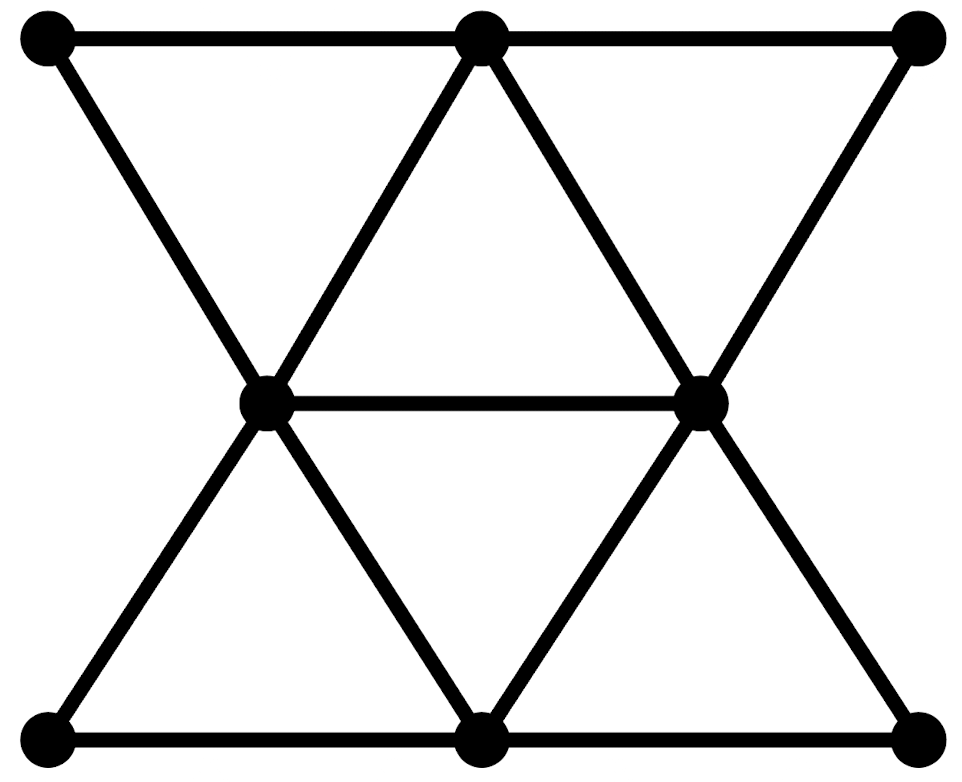
\includegraphics[width=\linewidth]{figure_source/triangulations/unlabeled/maximal/nonconvex.png}
		\caption{}
	\end{subfigure}\hspace{12pt}
	\begin{subfigure}{0.3\textwidth}
		\centering
		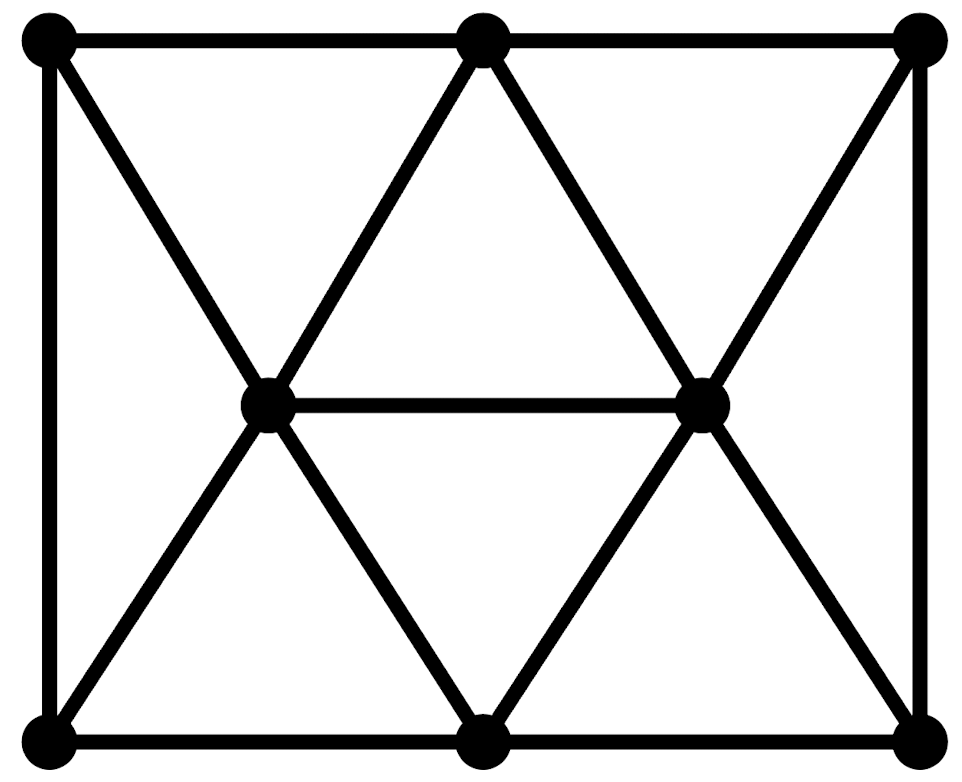
\includegraphics[width=\linewidth]{figure_source/triangulations/unlabeled/maximal/convex.png}
		\caption{}
	\end{subfigure}
	\caption{Two triangular meshes connecting the same set of points, showing the need for a maximal set.}
	\label{fig:triangulations.unlabeled.maximal}
\end{figure}
